\documentclass{book}
\usepackage{commeunjeustyle}
\begin{document}
\chapter{Équations différentielles ordinaires}
Les équations différentielles forment le langage dans lequel les lois fondamentales de
la science sont exprimées. La science nous dit comment le système actuel
change "d'un instant à l'autre". Le défi relevé par le
la théorie des équations différentielles est de prendre cette information à court terme
 et obtenir des informations sur le comportement général à long terme.
L'art et la pratique des équations différentielles implique cette
séquence d'étapes : on "modélise" un système (physique, chimique, biologique,
économique, voire mathématique) au moyen d'une équation différentielle ;
on tente ensuite d'obtenir des informations sur les solutions de cette équation ;
et on traduit ensuite cette information mathématique dans le
contexte scientifique.
\begin{center}
\setlength{\unitlength}{1cm}
\begin{picture}(5,4)(-3,-3)
\put(0,-3){\vector(-1,1){3}}
\put(0,-3){\vector(-1,1){3}}
\put(3,0){\vector( -1,-1){3}}
\put(-3,0) {\vector(1,0){6}}
\put(-0.75,-3.25){Monde physique}
\put(-8,0.1){Équation différentielle : temps courts}
\put(3,0.1){Solutions  : comportement dans le temps}
\put(-2.5,-1.5){Modélisation}
\put(1,-1.5){Interprétation}
\put(-0.5,0){Résolution}
\end{picture}
\end{center}
\begin{Exemple} Le problème est de déterminer l'angle d'un canon pour toucher une cible à la distance $l$.
\begin{itemize} 
\item \textit{Monde physique} :  trajectoire d'un boulet de canon.
\begin{center}
\includegraphics[width=6cm]{C7_equation_differentielle_parabole.png}
\end{center} 
\item \textit{Modélisation} :  La deuxième loi de Newton "Les changements qui arrivent dans le mouvement sont proportionnels à la force motrice ; et se font dans la ligne droite dans laquelle cette force a été imprimée." s'écrit : $$\sum \vec{F} = m\vec{a}$$ avec $\vec{a}$ l'accélération, la dérivée seconde de la position. L'unique force s'exerçant sur le point matériel $M$ est le poids en négligeant la force de frottement et la force de Coriolis.
\item \textit{Équation différentielle} : on obtient les équations différentielles suivantes :
 $$(E):x''(t) = 0 \text{ et } y''(t) = -g\quad  \text{ avec } x'(0)=v_0.\cos \alpha \text{ et } y'(0)=v_0.\sin \alpha.$$
\item \textit{Résolution} : par intégrations successives, on obtient la solution :
$$ x(t) = \cos \alpha .v_0. t  \text{ et } y(t) =  -\frac 1 2 g.t^2+v_0.\sin \alpha.t.$$
\item \textit{Solution} : $y$ vérifie une équation d'une parabole et pour $t_1=2  \frac{v_0.\sin \alpha. t}{g}$, on a $y(t_1) =0$. D'où $l=x(t_1) = \cos \alpha.v_0.2  \frac{v_0.\sin \alpha }{g}=\frac{v_0^2.\sin (\alpha/2)}{g}$, d'où $\alpha =\frac 1 2 \arcsin(\frac{lg}{v_0 ^2})$ si $\frac{lg}{v_0 ^2}\leq 1$ et pas de solution sinon.
\item  \textit{Interprétation} : si la longueur, $l$, est plus grande que $\frac{v_0 ^2}{g}$, alors le boulet de canon ne pourra pas atteindre sa cible, sinon l'angle doit être égale à  $\frac 1 2 \arcsin(\frac{lg}{v_0 ^2})$ 
\end{itemize}
\end{Exemple}
%\Para{Exemple 2} Évolution du nombre de noyaux radioactifs :
%$$(E):x'(t) = -\frac 1 k x(t).$$
% On résout analytiquement cette équation par séparation des variables. L'ensemble des solutions est  $$\mathcal{S}_\R    (E)=\{t\mapsto c e^{-\frac t k} :c\in \mathbb{R}\}.$$
%\begin{center}
%\includegraphics[width=6cm]{C7_equation_differentielle_radioactivite.png}
%\end{center}
Ce chapitre reprend rapidement et étend l'étude des équations différentielles linéaires vues en première année.\\
\textit{Notations :}
\begin{itemize}
\item $\K$ désigne le corps $\R$ ou $\C$,
\item $I$ désigne un intervalle (non vide et non réduit à un point) de $\R    $,
\item $J$ désigne un intervalle (non vide et non réduit à un point) \emph{inclus dans $I$},
\item toutes les fonctions qui interviennent sont (au moins) continues,
\item $t\in I$ est la variable par rapport à laquelle on dérive,
\item dans le cas scalaire, la fonction inconnue est $x \colon t \mapsto x(t)\in \K     $,
\item dans le cas vectoriel,
  \begin{itemize}
  \item on identifie $\mathcal{M}_{n1}(\K)$ et $\K^n$,
  \item la fonction inconnue est $X \colon t \mapsto X(t)\in \K^n$.
  \end{itemize}
\end{itemize}

%% -----------------------------------------------------------------------------
\section{Équations différentielles du premier ordre}
\subsection{Généralités}

\begin{Definition} Une \defi{équation différentielle de premier ordre} est une équation de la forme : 
$$F(t,x(t),x'(t))=0$$ où $F$ est une fonction quelconque.\\
Une \defi{solution sur $J\subset I$} de cette équation est une fonction $f$ de $J$ dans $\K$,
dérivable en tout point de $J$, telle que pour tout $t\in J$, on ait
\[F(t,f(t),f'(t)) = 0).\]
On note $\mathcal{S}_J(E)$ l'ensemble des solutions de $\mathrm{E}$ sur $J$.\\
\defi{Résoudre} $\mathrm{E}$, c'est déterminer $\mathcal{S}_J(E)$
pour tout intervalle $J\subset I$.\\
Les courbes représentatives des solutions de $\mathrm{E}$ s'appellent \defi{courbes intégrales} de $\mathrm{E}$.
\end{Definition}
\begin{Exemple}Considérons l'équation différentielle non linéaire $x'(t)+(x(t))^2=t^2.$ 
\begin{center}
\includegraphics[width=6cm]{C7_equation_differentielle_unresolded.png}
\end{center}
\end{Exemple}
%
\begin{Definition}[Normalisée]  Une équation différentielle de premier ordre est  dite \defi{normalisée} ou \defi{résolue en $x'$}
  si elle est de la forme  $$x'(t) =F(t,x(t))$$
où $F$ est une fonction quelconque.
\end{Definition}
\subsection{Approximations de l'équation résolue $x'(t)=F(t,x(t))$ }
L'équation différentielle $ x'(t)+(x(t))^2=t^2$ n'admet pas de résolution analytique à l'aide des fonctions usuelles. L'approche géométrique et numérique sont des procédés pour déterminer des approximations des solutions exactes. 
 
\subsubsection{Approche géométrique}
Comme l'équation $x'(t) = F(t,x(t))$ spécifie la dérivée, soit la pente à chaque point $(t,x)$ du plan, on connaît ainsi la pente des fonctions solutions, $x$. Le \defi{champ des
directions} de l'équation différentielle est un graphe  représentant par des petits segments  les dérivées tangentes à la trajectoire en différents points. En partant d'un point $(t_0,x_0)$ on peut tracer la courbe intégrale par approximation en suivant le champ des directions. On obtient une approximation de la solution particulière $x$ qui satisfait à la condition initiale $x(t_0)=x_0$.

Pour tracer à la main le champs des directions par un humain, l'algorithme est :
\begin{enumerate}
\item  Choisir une pente $c$
\item  Résoudre l'équation $F(t,x)=c$
\item  Tracer la solution.
\end{enumerate}
\begin{Exemple}[Cercle] On considère l'équation différentielle $(E):\quad x'(t) = -\frac{t}{x(t)}$.\\
Pour $c=1$, on obtient l'équation de droite $x=-t$.\\
Pour $c=-1$, on obtient l'équation de droite $x=t$.\\
Pour $c=0$, on obtient l'équation de droite $t=0$.\\
Pour $"c=\infty"$, on obtient l'équation de droite $x=0$.
\begin{center}
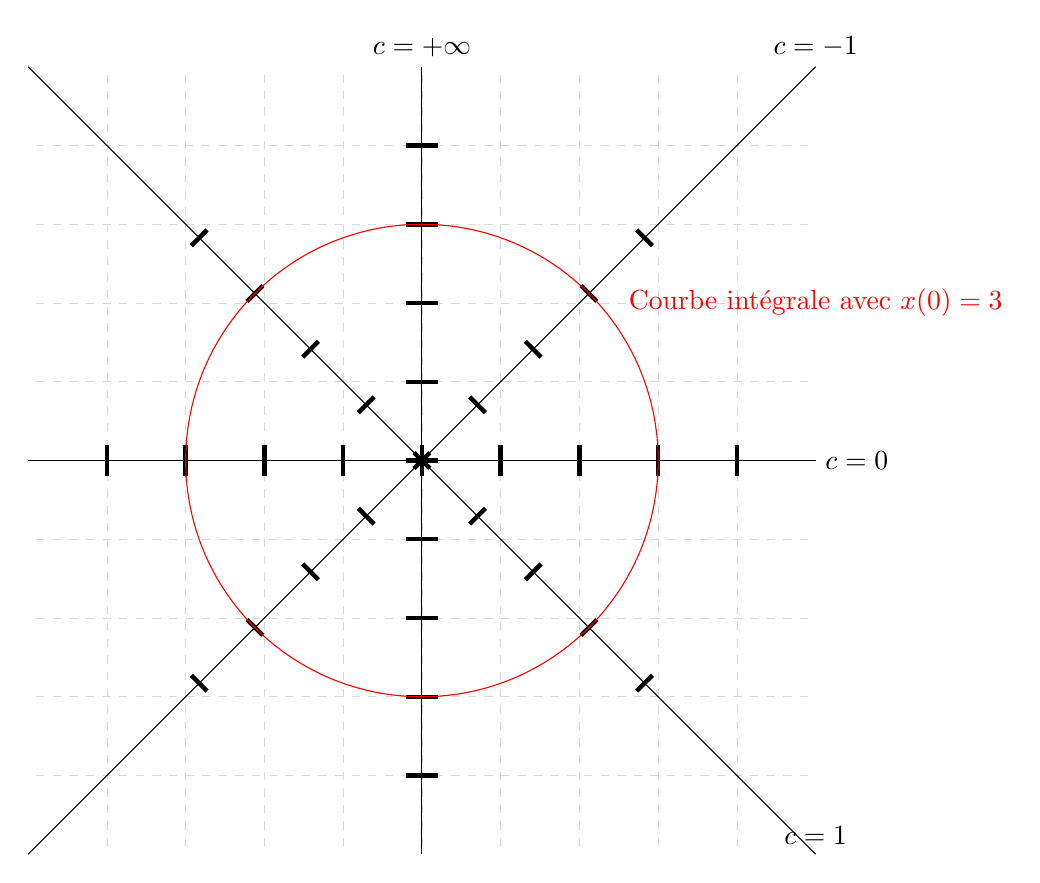
\begin{tikzpicture}
\draw[help lines, color=gray!30, dashed] (-4.9,-4.9) grid (4.9,4.9);
\draw (-5,0)--(5,0) node[right]{$c=0$};
\foreach \x in {-4,-3,-2,-1,0,1,2,3,4} \draw[ultra thick] (-0.2,\x) -- (0.2,\x);
\draw (0,-5)--(0,5) node[above]{$c=+\infty$};
\foreach \x in {-4,-3,-2,-1,0,1,2,3,4} \draw[ultra thick] (\x,-0.2) -- (\x,0.2);
\draw (-5,-5)--(5,5) node[above]{$c=-1$};
\foreach \x in {-4*0.707,-3*0.707,-2*0.707,-1*0.707,0,1*0.707,2*0.707,3*0.707,4*0.707} \draw[ultra thick] (\x-0.1,\x+0.1) -- (\x+0.1,\x-0.1);
\draw (-5,5)--(5,-5) node[above]{$c=1$};
\foreach \x in {-4*0.707,-3*0.707,-2*0.707,-1*0.707,0,1*0.707,2*0.707,3*0.707,4*0.707} \draw[ultra thick] (-\x-0.1,\x-0.1) -- (-\x+0.1,\x+0.1);
\draw[color=red] (0,0) circle (3);
\draw (5,2) node{\color{red}Courbe intégrale avec $x(0)=3$};
\end{tikzpicture}
\end{center}
On observe que l'ensemble des solutions sont les cercles centrées en 0.
\end{Exemple}
Pour tracer numériquement le champs des directions par un humain, l'algorithme est :
\begin{enumerate}
\item Choisir des points $(t,x)$ régulièrement espacés
\item Calculer $F(t,x)$
\item Tracer un segment de droite de pente $F(t,x)$ au point $(t,x)$
\end{enumerate}
\begin{Exemple} On considère l'équation $(E):x'(t)=1+t-x(t)$.\\
\begin{center}
\includegraphics[width=9cm]{C7_equation_differentielle_solution.png}
\end{center}
On observe que le comportement asymptotique de la trajectoire est $x(t)\underset{\infty}{\sim} t$. Aussi les courbes intégrables partitionnent le plan (une unique courbe intégrable passe en chaque point du plan) donc on peut conjecturer l'existence et l'unicité d'une solution ayant une condition initiale $x(t_0)=x_0$.
\end{Exemple}
\subsubsection{Approche  numérique}
La méthode d'Euler permet d'obtenir une approximation d'une solution particulière d'une équation différentielle donnée par $(E):x'(t)=F(t,x(t))$.\\
A partir d'un point $(t_0,x_0)$, on suit géométriquement \footnote{De manière analytique, on a $$ \lim_{h\to 0}\frac{x(t+h)-x(t)}{h}=x'(t)=F(t,x).$$ Donc, si $h<<1$, on peut approximer 
$$ \frac{x(t+h)-x(t)}{h}\approx F(t,x).$$D'où $$ x(t+h)\approx x(t) +  h.F(t,x).$$ Soit $x_1=x_0+h.F(t_0,x_0)$.} la pente $p$ du champs de direction donnée par l'équation différentielle $p=x'(t_0)=F(t_0,x_0)$.
Ainsi, à partir du point on obtient un deuxième point $(t_1,x_1)$ avec $t_1=t_0+h$ et $x_1=x_0+h.p$ , où $h$ est un pas fixé d'avance.
En continuant ainsi, on obtient une suite de points qui approchent la courbe intégrale passant par  $(t_0,x_0)$.
\begin{Exemple}[Bosse]  On considère l'équation différentielle $(E):\quad x'(t) = -2.t.x(t)$. 
\begin{center}
\includegraphics[width=8cm]{C7_equation_differentielle_bosse.png}
\end{center}
\end{Exemple}
\subsection{Résolution analytique : le cas linéaire}
\subsubsection{Cadre}
\begin{Definition}
Une \defi{équation différentielle linéaire scalaire du premier ordre}
est une équation de la forme
\[\tag{$\mathrm{E}$} a(t) x'(t) + b(t) x(t) = c(t),\]
où $a$, $b$ et $c$ sont des fonctions continues de $I$ dans $\K     $,
et $x$ une fonction inconnue de $I$ dans $\K$.\\
$\mathrm{E}$ est dite \defi{à coefficients constants}
  si les fonctions $a$ et $b$ sont constantes.\\
$\mathrm{E}$ est dite \defi{homogène} ou \defi{sans second membre}
  si  $  c(t) = 0$ pour tout $t$.\\
On appelle \defi{équation différentielle homogène associée} à $\mathrm{E}$
  ou \defi{équation différentielle sans second membre associée} à $\mathrm{E}$
  l'équation différentielle
 \[\tag{$\mathrm{E_0}$} a(t) x'(t) + b(t) x(t) = 0.\]
\end{Definition}
\begin{Remarque}
Si $a$ ne s'annule pas sur $I$, l'ensemble des solutions de l'équation différentielle (E) est égale à l'ensemble des solutions de l'équation différentielle normalisée :
\[\tag{$\mathrm{E}$}  x'(t) + \frac{b(t)}{a(t)} x(t) = \frac{c(t)}{a(t)}.\]
\end{Remarque}

\begin{Definition}[Problème de Cauchy]
Un \defi{problème de Cauchy} du premier ordre
est la donnée d'une équation différentielle du premier ordre
normalisée et d'une condition initiale.\\
Un problème de Cauchy linéaire du premier ordre est donc de la forme
\[\tag{$\mathrm{C}$} \begin{cases}
    \forall t\in I:\quad x'(t) + b(t)x(t) = c(t), \\
    x(t_0) = x_0 \text{ où } t_0\in I \text{ et } x_0\in \K     .
\end{cases}.\]
\end{Definition}
\subsubsection{Étude théorique}
\begin{Proposition}
Soit $f$ une solution sur $J$ de l'équation différentielle normalisée
\[\tag{$\mathrm{E}$} x'(t) + b(t) x(t) = c(t).\]
Alors $f$ est de classe $C^1$ sur $J$.\\
De plus, si $b$ et $c$ sont de classe $C^ p$ sur $J$,
alors $f$ est de classe $C^{p+1}$ sur $J$;
si $b$ et $c$ sont de classe $C^{\infty}$ sur $J$, alors $f$ l'est également.
\end{Proposition}
\begin{Theoreme}[Cauchy-Lipschitz linéaire]
Soit $b:I\to \K     $ et $c:I\to \K     $ deux fonctions continues.\\
Soit $t_0\in I$ et $x_0\in \K$.\\
Alors le problème de Cauchy
\[\tag{$\mathrm{C}$}
  \begin{cases}
    \forall t\in I:\quad  x'(t) + b(t) x(t) = c(t), \\
    x(t_0) = x_0
\end{cases}\]
admet une unique solution sur tout intervalle $J$ tel que $t_0\in J$ et $J\subset I$.\\
De plus, la solution sur $J$ n'est autre que la restriction à $J$
de la solution sur $I$.
\end{Theoreme}
\begin{Corollaire}[Partition du plan]
Soit $\mathrm{E}$ une équation différentielle linéaire scalaire normalisée
du premier ordre sur $I$
\[\tag{$\mathrm{E}$} x'(t) + b(t)x(t) = c(t).\]
Alors les courbes intégrales de $\mathrm{E}$ sont disjointes.\\
Plus précisément, elles forment une partition de $I\times\R$.
\begin{center}
\includegraphics[width=8cm]{C7_equation_differentielle_partition.png}\\
Partition du plan par les solutions de l'équation $x'(t)=1+t-x(t)$.
\end{center}
\end{Corollaire}
\begin{Demonstration}
Du fait de l'unicité du théorème de Cauchy-Lipschitz linéaire, les courbes intégrales sont disjointes.\\
Du fait de l'existence, une courbe intégrale passe en chaque point du plan.
\end{Demonstration}
\begin{Corollaire}
Soit $f$ une solution sur $J$ de l'équation différentielle linéaire scalaire
normalisée homogène du premier ordre
\[\tag{$\mathrm{E_0}$} x'(t) + b(t) x(t) = 0.\]
Alors
\begin{itemize}
\item soit $f$ est identiquement nulle sur $J$,
\item soit $f$ ne s'annule pas sur $J$.
\end{itemize}
\end{Corollaire}
\begin{Demonstration}
Supposons que $f$ s'annule sur $J$, soit $f(x_0)=0$. Comme la fonction nulle est solution de $(E_0)$ et passe par le point $(x_0,0)$, d'après l'unicité de la solution du théorème Cauchy-Lipschitz linéaire, $f=0$. 
\end{Demonstration}


\begin{Theoreme}[Structure]
On considère les équations différentielles linéaires scalaires
normalisées du premier ordre 
\[\tag{$\mathrm{E}$}   x'(t) + b(t)x(t) = c(t)\]
\[\tag{$\mathrm{E_0}$} x'(t) + b(t)x(t) = 0\]
\begin{itemize}
\item $\mathcal{S}_J(E_0)=Vect(t\mapsto e^{-B(t)})$ sous-espace vectoriel de dimension $1$ avec $B$ primitive de $b$.
\item $\mathcal{S}_J(E) = x_p +Vect(t\mapsto e^{-B(t)})$, sous-espace affine de dimension $1$ avec $x_p$ une solution particulière.
\end{itemize}
\end{Theoreme}
La \og{}résolution\fg{} suivante peut permettre de retrouver la formule
\begin{enumerate}
\item $x'(t) + b(t) x(t) = 0$
\item $\frac{x'(t)}{x(t)} = -b(t)$
\item $\ln\|x(t)\| = -B(t) + C_0$ où $C_0\in \R    $
\item $x(t) = K e^{-B(t)}$ où $K\in \R    $
\end{enumerate}
Néanmoins, \impo{il ne s'agit pas d'une preuve} à cause
\begin{itemize}
\item de la division par $x(t)$ qui pourrait s'annuler, et
\item du passage de $\|x(t)\|$ à $x(t)$ nécessite des justifications
  (on pourrait imaginer que $x$ change de signe et donc que $K$ soit une fonction de $t$...)
\end{itemize}
Bref, à éviter sur une copie, sauf si l'on sait déjà que $\forall x\in I$, $x(t)>0$.

\begin{Exemple}[Charge d'un condensateur d'un circuit RC]
La tension d'un circuit RC en charge est gouvernée par l'équation différentielle  :
\[\tag{$\mathrm{E}$}   RC u'(t) + u(t) = E\]
soit, en posant $\tau =RC$, 
\[\tag{$\mathrm{E}$}   u'(t) + \frac 1 \tau u(t) = \frac E \tau\]
L'ensemble des solution est  :
$$ t\mapsto E + \lambda e^{t/\tau}\text{ avec } \lambda \in \R.$$
\end{Exemple}

\subsubsection{En pratique}
\paragraph{Principe de superposition}
Si $\mathrm{E}$ est de la forme
\[\tag{$\mathrm{E}$} a(t) x'(t) + b(t) x(t) = c_1(t) + c_2(t),\]
pour trouver une solution particulière de $\mathrm{E}$, il suffit de
\begin{itemize}
\item trouver une solution particulière $x_{p,1}$ de
  \[\tag{$\mathrm{E_1}$} a(t) x'(t) + b(t) x(t) = c_1(t),\]
\item trouver une solution particulière $x_{p,2}$ de
  \[\tag{$\mathrm{E_2}$} a(t) x'(t) + b(t) x(t) = c_2(t),\]
\item poser $x_p = x_{p,1} + x_{p,2}$.
\end{itemize}
Dans ces conditions, $x_p$ est une solution particulière de $\mathrm{E}$.

\paragraph{Recherche d'une solution particulière d'une équation à coefficients constants}

On considère l'équation différentielle
\[\tag{$\mathrm{E}$} x'(t) + ax(t) = P(t) e^{\alpha t},\]
où $P\in \K_d[X]$.
Il existe une unique solution particulière de la forme
\begin{enumerate}
\item Si $\alpha\neq -a$, on prend $x_p(t) = Q(t) e^{\alpha t}$
  où $Q\in \K     _d[X]$ à déterminer.
\item Si $\alpha= -a$, on prend $x_p(t) = tQ(t) e^{\alpha t}$
  où $Q\in \K     _d[X]$ à déterminer.
\end{enumerate}
Bien sûr, si le second membre est une somme de termes de ce type,
il suffit de superposer les solutions particulières correspondantes.
\begin{Exemple}
\begin{enumerate}
\item Pour $x' + x = te^t$, on prend $x_p = (at+b)e^t$.
\item Pour $x' - x = (t+1)e^t$, on prend $x_p = t(at+b)e^t$.
\item Pour $x' + x = \sin t$, on prend $x_p = a\cos t + b\sin t$.
\item Pour $x' + 3x = t\cos 2t$, on prend $x_p = (at+b)\cos 2t + (ct+d)\sin 2t$.
\item Pour $x' + x = te^t - e^{2t}$, on prend $x_p = (at+b)e^t + ce^{2t}$.
\end{enumerate}
\end{Exemple}
\paragraph{Recherche d'une solution particulière  par la méthode de variation de la constante}
On considère les équations différentielles
\[\tag{$\mathrm{E}$}   x'(t) + a(t) x(t) = b(t),\]
\[\tag{$\mathrm{E_0}$} x'(t) + a(t) x(t) = 0.\]
Soit $\phi  $ une solution non nulle de $\mathrm{E_0}$ sur $J$.
On rappelle que $\phi  $ ne s'annule pas et que
la solution générale de $\mathrm{E_0}$ est donnée par
\[x_0(t) = K\phi  (t) \quad \text{où } K\in \K     .\]
On recherche alors les solutions de $\mathrm{E}$ sous la forme
$x(t) =k(t)\phi  (t)$, et l'on obtient
\[\tag{$\mathrm{E'}$}k'(t)\phi  (t) = b(t),\]
qui est facile à résoudre.

\begin{Corollaire}
La solution du problème de Cauchy
\[\begin{cases}
    \forall t\in I:\quad x'(t) + a(t)x(t) = b(t), \\
    x(t_0) = x_0
\end{cases}\]
est donnée par
\[x(t) = e^{-A(t)} \left( e^{A(t_0)} x_0 + \int_{t_0}^{t} e^{A(u)}b(u) \mathrm{du} \right),\]
où $A$ est une primitive de $a$ sur $I$.
Cette formule \emph{n'est pas à connaître}, mais à savoir retrouver au besoin.
\end{Corollaire}
\subsubsection{Raccordement}

Étant donné l'équation différentielle linéaire scalaire du premier ordre
\[\tag{$\mathrm{E}$} a(t) x'(t) + b(t) x(t) = c(t),\]
on peut se ramener à une équation normalisée:
\begin{enumerate}
\item si $a$ ne s'annule pas sur $I$, il suffit de diviser par $a(t)$;
\item par contre, si $a$ s'annule, on découpe $I$ en intervalles
  où $a$ ne s'annule pas, puis on fait une étude sur chaque intervalle.
  À la fin, on cherche à \og{}raccorder\fg{} les solutions.
\end{enumerate}
Supposons par exemple que $I=\R    $ et que $a$ s'annule uniquement en $0$.
\begin{itemize}
\item On pose alors $I_1 = ]-\infty,0[$ et $I_2 = ]0,+\infty[$.
  Sur ces deux intervalles, $\mathrm{E}$ est une équation normalisée, donc
  on peut la résoudre.
\item On résout $\mathrm{E}$ sur $I_1$ et sur $I_2$.
\item On détermine, généralement par la méthode d'analyse-synthèse,
  quelles sont les fonctions $f$
  solutions de $\mathrm{E}$ sur $\R $, sachant que la restriction de $f$ à $I_k$
  est nécessairement une solution de $\mathrm{E}$ sur $I_k$.
\end{itemize}

\begin{Exemple}  On considère l'équation différentielle $(E):\quad tx'(t)  -x(t)=0$ définie sur $\mathbb{R}$. 
\begin{center}
\includegraphics[width=8cm]{C7_equation_differentielle_raccord2.png}\\
On observe que les courbes intégrables s'intersectent et ne sont pas tangentes en l'origine.
\end{center}
Résolution analytique : on cherche à « recoller » certaines de ces solutions de façon à obtenir des fonctions continues et dérivables sur
l'intervalle $\mathbb{R}$.\\
Pour appliquer les résultats de l'étude précédente à cette équation, on commence par la mettre sous la forme normalisée
$$ x'(t)  -\frac{1}{t}x(t)=0,$$
qui en limite l'étude à chacun des intervalles $\mathbb{R}^-$ et $\mathbb{R}^+$. Sur chacun de ces intervalles, les solutions sont
de la forme $t \mapsto at^2, a \in  \mathbb{R}$.

Cherchons, s'il en existe, les solutions définies sur $\mathbb{R}$ de cette équation.
\begin{itemize}
\item \textit{Analyse :} si $\phi  $ est une telle solution, alors c'est aussi une solution de l'équation $(E)$ sur chacun des
intervalles $\mathbb{R}^-$ et $\mathbb{R}^+$, donc il existe deux scalaires $a_1$ et $a_2$ tels que
$$\forall t < 0, \phi  (t) = a_1 t\text{ et } \forall t > 0, \phi  (t) = a_2 t.$$
Cette fonction doit être continue en 0, ce qui n'impose aucune restriction sur $a_1$ et $a_2$ et on a $\phi  (0) = 0$.\\
La fonction doit être dérivable en 0. On a alors :
$$\lim_{t\to 0^+} \frac{\phi  (t) - \phi  (0)}{t - 0}= \lim_{t\to 0^+}a_2 \frac{t}{t}=a_2 \text{ et } \lim_{t\to 0^-} \frac{\phi  (t) - \phi  (0)}{t - 0}= \lim_{t\to 0^-}a_1 \frac{t}{t}=a_1.$$
ce qui montre que les coefficients $a_1=a_2$, et que la fonction $\phi  $ ainsi construite est dérivable.\\
\item  \textit{Synthèse} : pour tout réel $a$, la fonction $\phi  $ définie par
$$\phi  (t) =a t  $$
est solution de l'équation différentielle sur $\mathbb{R}$.
\end{itemize}
\end{Exemple}
\begin{Exemple}   On considère l'équation différentielle $(E):\quad tx'(t)  -2.x(t)=0$ définie sur $\mathbb{R}$. 
\begin{center}
\includegraphics[width=8cm]{C7_equation_differentielle_raccord.png}\\
On observe que les courbes intégrables s'intersectent et sont tangentes en l'origine.
\end{center}
Résolution analytique : on cherche à « recoller » certaines de ces solutions de façon à obtenir des fonctions continues et dérivables sur
l'intervalle $\mathbb{R}$.\\
Pour appliquer les résultats de l'étude précédente à cette équation, on commence par la mettre sous la forme normalisée
$$ x'(t)  -\frac{2}{t}x(t)=0,$$
qui en limite l'étude à chacun des intervalles $\mathbb{R}^-$ et $\mathbb{R}^+$. Sur chacun de ces intervalles, les solutions sont
de la forme $t \mapsto at^2, a \in  \mathbb{R}$.

Cherchons, s'il en existe, les solutions définies sur $\mathbb{R}$ de cette équation.\\
\textit{Analyse :} si $\phi  $ est une telle solution, alors c'est aussi une solution de l'équation $(E)$ sur chacun des
intervalles $\mathbb{R}^-$ et $\mathbb{R}^+$, donc il existe deux scalaires $a_1$ et $a_2$ tels que
$$\forall t < 0, \phi  (t) = a_1 t^2\text{ et } \forall t > 0, \phi  (t) = a_2 t^2.$$
Cette fonction doit être continue en 0, ce qui n'impose aucune restriction sur $a_1$ et $a_2$ et on a $\phi  (0) = 0$.\\
La fonction doit être dérivable en 0. On a alors :
$$\lim_{t\to 0^+} \frac{\phi  (t) - \phi  (0)}{t - 0}= \lim_{t\to 0^+}a_2 \frac{t^2}{t}=0 \text{ et } \lim_{t\to 0^-} \frac{\phi  (t) - \phi  (0)}{t - 0}= \lim_{t\to 0^-}a_1 \frac{t^2}{t}=0.$$
ce qui montre que les coefficients $a_1$ et $a_2$ peuvent être choisis de façon arbitraire, non nécessairement
égaux, et que la fonction $\phi  $ ainsi construite est dérivable.\\
\textit{Synthèse} : pour tous réels $a_1$, $a_2$, la fonction $\phi  $ définie par
$$\phi  (t) =\begin{cases}a_2 t &\text{si }t<0 \\0 &\text{si }t=0\\ a_1 t &\text{si }t>0\end{cases}\text{ avec } a_1, a_2 \in  \mathbb{R} $$
est solution de l'équation différentielle sur $\mathbb{R}$ (et ce sont les seules). En particulier, les fonctions de la forme $t \mapsto a t^2$
sont des solutions de l'équation, mais ce ne sont pas les seules.

\begin{center}
\includegraphics[width=8cm]{C7_equation_differentielle_raccord3.png}\\
La condition initiale $(t_0=-2,x_0=-4)$ impose la courbe rouge correspond au $t<0$. En revanche, pour les $t>0$, une courbe intégrable est une parabole passant par l'origine, par exemple les courbes verte ou violet ou bleu . Il n'y a pas unicité de la solution.  De plus, si la condition initial est $x(0)\neq 0$, il n'y a pas existence d'une solution. 
\end{center}
\end{Exemple}
\begin{Proposition}[Problème de Cauchy]
Soit $a:I\to \K     $,  $b:I\to\K     $ et $c:I\to\K     $ trois fonctions continues.\\
Soit $t_0\in I$ et $x_0\in \K$.\\
Alors le problème 
\[\tag{$\mathrm{C}$}
  \begin{cases}
    \forall t\in I:\quad a(t)x'(t) + b(t) x(t) = c(t), \\
    x(t_0) = x_0
\end{cases}\]
n'admet pas nécessairement une solution sur tout intervalle $J$ et si elle existe et n'est pas nécessairement unique (voir le second exemple sur le raccordement).
\end{Proposition}
%% -----------------------------------------------------------------------------
\section{Systèmes différentiels linéaires}
On étudie le mouvement d'un système de deux masses reliées par des ressorts, glissant le long d'une poutre soufflante.
\begin{center}
\includegraphics[width=12cm]{resort.png}
\end{center}
Pour simplifier, les ressorts ont même raideur k et les corps même masse m.
Notons $x_i(t)$ l'écart par rapport à la position d'équilibre pour le i-ème corps.\\
Le principe fondamentale de la dynamique s'écrit :
$$m x_1''(t) = -2k.x_1(t)  +k.x_2(t)$$
$$m x_2''(t) = k.x_1(t)  - 2k.x_2(t)$$
On peut alors le mettre sous la forme $ X''(t)= AX(t)$
 avec :
 $$X(t)=\begin{pmatrix} x_1(t)\\x_2(t) \end{pmatrix}\in \M{2}{1}{\R}\text{ et }A=\frac k m \begin{pmatrix}
 -2&1\\1&-2\\
 \end{pmatrix}\in\M{2}{2}{\R} $$
Les physiciens ont compris qu'en général, le mouvement est une superposition de mouvements
fondamentaux appelés modes propres. Ce sont les mouvements où tous les corps oscillent à la
même fréquence. Dans ce système, les fréquence propres sont les racine carré de l'opposé des valeurs propres  de $A$, soit $\sqrt{\frac{k}{m}}$ et $\sqrt{3\frac{k}{m}}$.
\subsection{Généralités}
\begin{Definition}
Un \defi{système différentiel linéaire du premier ordre} est une équation de la forme
\[\tag{$\mathrm{S}$} X'(t) = A(t) X(t) + B(t)\]
où $A:I\to \MnK$ et $B: I\to \M{n}{1}{\K}$ sont des fonctions continues,
et $X: I\to \M{n}{1}{\K}$ est une fonction inconnue.\\
Une \defi{solution sur $J\subset I$} de ce système est une fonction $f$ de $J$ dans $\M{n}{1}{\K}$,
dérivable en tout point de $J$, telle que pour tout $t\in J$, on ait
\[f'(t) = A(t) f(t) + B(t).\]
On note $\mathcal{S}_J(S)$ l'ensemble des solutions de $\mathrm{S}$ sur $J$.\\
\defi{Résoudre} $\mathrm{S}$, c'est déterminer $\mathcal{S}_J(S)$ pour tout intervalle $J\subset I$.
\begin{itemize}
\item $\mathrm{S}$ est dit \defi{à coefficients constants}
  si  la fonction $A$ est constante.
\item $\mathrm{S}$ est dit \defi{homogène} ou \emph{sans second membre}
  si \[\forall t\in I :\quad B(t) = 0.\]
  \item On appelle \defi{système différentiel homogène associe} à $\mathrm{S}$
  le système différentiel
  \[\tag{$\mathrm{S_0}$} X'(t) = A(t) X(t).\]
\end{itemize}
\end{Definition}
\begin{Definition}[Problème de Cauchy]
Un \defi{problème de Cauchy} du premier ordre est la donnée d'un système différentiel linéaire du premier ordre
et d'une condition initiale.\\
Un problème de Cauchy linéaire du premier ordre est donc de la forme
\[\tag{$\mathrm{C}$} \begin{cases}
    \forall t\in I:\quad X'(t) = A(t)X(t) + B(t), \\
    X(t_0) = X_0 \text{ où $t_0 \in I$ et $X_0\in \K     $.}
\end{cases}\]
\end{Definition}
\subsection{Étude théorique}
\begin{Proposition}
Soit $f$ une solution sur $J$ du système différentiel
\[\tag{$\mathrm{S}$} X'(t) = A(t) X(t) + B(t).\]
Alors $f$ est de classe $C^1$ sur $J$.\\
De plus, si $B$ et $C$ sont de classe $C^ p$ sur $J$,
alors $f$ est de classe $C^{p+1}$ sur $J$;
si $B$ et $C$ sont de classe $C^{\infty}$ sur $J$, alors $f$ l'est également.
\end{Proposition}
\begin{Theoreme}[Cauchy-Lipschitz linéaire]
Soit $A:I\to\MnK$ et $B:I\to \M{n}{1}{\K}$ deux fonctions \emph{continues}.\\
Soit $t_0\in I$ et $X_0\in \M{n}{1}{\K}$.\\
Alors le problème de Cauchy
\[\tag{$\mathrm{C}$} \begin{cases}
    \forall t\in I:\quad X'(t) = A(t) X(t) + B(t), \\
    X(t_0) = X_0
\end{cases}\]
admet une unique solution sur tout intervalle $J$ tel que $t_0\in J$ et $J\subset I$.\\
De plus, la solution sur $J$ n'est autre que la restriction à $J$
de la solution sur $I$.
\end{Theoreme}
%\Para{Proposition}
%
%Soit $t_0\in J$.
%On considère le système différentiel homogène
%\[\tag{$\mathrm{S_0}$} X'(t) = A(t)X(t)\]
%Alors l'application
%\[\Fonction{\phi  }{\mathcal{S}_J(S_0)}{\K     ^n}{X}{X(t_0)}\]
%est un isomorphisme (c.-à-d. une application linéaire bijective).
%
\begin{Theoreme}[Structure]
On considère les systèmes différentiels linéaires
\[\tag{$\mathrm{S}$}   X'(t) = A(t)X(t) + B(t)\]
\[\tag{$\mathrm{S_0}$} X'(t) = A(t)X(t)\]
Alors:
\begin{itemize}
\item $\mathcal{S}_J(S_0)$ est un sous-espace vectoriel de $C^1(I,\M{n}{1}{\K})$ de dimension $n$.
\item $\mathcal{S}_J(S)$ est un sous-espace \emph{affine} de $C^1(I,\M{n}{1}{\K})$ de dimension $n$ et de direction $\mathcal{S}_J(S_0)$.
\end{itemize}
\end{Theoreme}
\subsection{Résolution pratique $X'(t)=AX(t)$}
\subsubsection{$A$ diagonalisable dans $\Mn{\R}$}
Considérons le système $\begin{cases}x_1'(t)=&-2x_1(t)+x_2(t)\\x_2'(t)=&x_1(t)-2x_2(t) \end{cases}$ qui s'écrit sous forme matricielle :
$$X'(t)=AX(t)\text{ avec } X(t)=\begin{pmatrix}x_1(t)\\x_2(t)\end{pmatrix}\text{ et }A=\begin{pmatrix}-2&1\\1&-2\end{pmatrix}.$$
La matrice A est diagonalisable dans $\R$ car symétrique à coefficients réels. On trouve que 
$$ A=PDP^{-1}\text{ avec } P=\begin{pmatrix}1 &1\\1&-1\\ \end{pmatrix}\text{ et }D=\begin{pmatrix}-1 &0\\0&-3\\ \end{pmatrix}.$$
L'idée est de ramener la résolution du système $X'(t) = AX(t)$  à celle d'un système   $Y'(t)=DY(t)$, où  $D$ est diagonale. On a 
$$X'=AX\Leftrightarrow X'=PDP^{-1}X\Leftrightarrow  P^{-1}X'=DP^{-1}X\Leftrightarrow  Y'=DY \text{ avec } Y=P^{-1}X  $$
$Y'=(P^{-1}X)'=P^{-1}X'$ car les coefficient de $P^{-1}$ ne dépendent pas de $t$.
Le nouveau système obtenue est  $\begin{cases}y_1'(t)=&-y_1(t)\\y_2'(t)=&-3y_2(t) \end{cases}$, soit $\begin{cases}y_1(t)=&k_1 e^{-t}\\y_2(t)=&k_2 e^{-3t} \end{cases}$ avec $k_1,k_2\in\R$.\\
Comme $X=PY$, on obtient 
$\begin{pmatrix}
x_1(t)\\x_2(t)
\end{pmatrix} = k_1e^{-t}\begin{pmatrix}
1\\1
\end{pmatrix}+k_2e^{-3t}\begin{pmatrix}
1\\-1
\end{pmatrix}$, soit   $\begin{cases}x_1(t)=&k_1 e^{-t}+k_2 e^{-3t}\\x_2(t)=&k_1 e^{-t}-k_2 e^{-3t} \end{cases}$ avec $k_1,k_2\in\R$.\\
On généralise facilement le résultat précédent à une matrice diagonalisable dans $\Mn{\R}$ quelconque.
\begin{Theoreme}
Soit $A\in \MnK$ et $X:\R\to\M{n}{1}{\K}$ une solution de
\[\tag{$\mathrm{S}$} X'(t) = A X(t).\]
On suppose que $A$ est diagonalisable : soit $(X_1,\dots X_n)$ une base de vecteurs propres associés aux valeurs propres $(\lambda_1,\dots,\lambda_n)$.\\
Alors il existe $k_1,\dots k_n \in \K$ tel que
\[\forall t\in \R   :\quad X(t) = \sum_{k=1}^n a_k e^{\lambda_k t} X_k.\]
\end{Theoreme}
\subsubsection{$A$ diagonalisable dans $\Mn{\C}$}
Considérons le système $\begin{cases}x_1'(t)=&3x_1(t)-2x_2(t)\\x_2'(t)=&3x_1(t)+1x_2(t) \end{cases}$ qui s'écrit sous forme matricielle :
$$X'(t)=AX(t)\text{ avec } X(t)=\begin{pmatrix}x_1(t)\\x_2(t)\end{pmatrix}\text{ et }A=\begin{pmatrix}3&-2\\3&1\end{pmatrix}.$$
La matrice A est diagonalisable dans $\C$ car le polynôme caractéristique $\chi_A=(X-(2+i\sqrt{5}))(X-(2-i\sqrt{5}))$ est scindé et simple. On trouve que 
$$ A=PDP^{-1}\text{ avec } P=\begin{pmatrix}1 & 1\\\frac{1-i\sqrt{5}}{2}& \frac{1+i\sqrt{5}}{2}\\ \end{pmatrix}\text{ et }D=\begin{pmatrix}2+i\sqrt{5} &0\\0&2-i\sqrt{5}\\ \end{pmatrix}.$$
Après avoir résolue le système différentielle en posant $X=PY$, on obtient :
$$\begin{pmatrix}
x_1(t)\\x_2(t)
\end{pmatrix} = k_1e^{(2+i\sqrt{5})t}\begin{pmatrix}
1\\\frac{1-i\sqrt{5}}{2}
\end{pmatrix}+k_2e^{(2-i\sqrt{5})t}\begin{pmatrix}
1\\\frac{1+i\sqrt{5}}{2}
\end{pmatrix}\text{ avec }k_1,k_2\in\C. $$ Or, 
$$e^{(2+i\sqrt{5})t}\begin{pmatrix}
1\\\frac{1-i\sqrt{5}}{2}
\end{pmatrix}=e^{2t}(\cos(\sqrt{5}t)+i\sin(\sqrt{5}t) )\begin{pmatrix}
1\\\frac{1-i\sqrt{5}}{2}
\end{pmatrix} =e^{2t}\begin{pmatrix}
\cos(\sqrt{5} t)\\  \cos(t) -\sqrt{5}\sin(\sqrt{5} t)\end{pmatrix}+i  e^{2t}\begin{pmatrix}
\sin(\sqrt{5} t)\\  \sin(t)+\sqrt{5}\cos(\sqrt{5} t)
\end{pmatrix}  $$ 
Malgré le détour par $\C$,  les solutions trouvées doivent être réelles.  On obtient :
$$\begin{pmatrix}
x_1(t)\\x_2(t)
\end{pmatrix} = ae^{2t}\begin{pmatrix}
\cos(\sqrt{5} t)\\  \cos(t) -\sqrt{5}\sin(\sqrt{5} t)\end{pmatrix} + b  e^{2t}\begin{pmatrix}
\sin(\sqrt{5} t)\\  \sin(t)+\sqrt{5}\cos(\sqrt{5} t)
\end{pmatrix}.$$
\subsubsection{$A$ trigonalisable dans $\Mn{\C}$}

Si $A$ est seulement la trigonalisable, on obtient : 
$A = P T P^{-1}$, on pose $X(t) = P Y(t)$, et le système devient
\[\tag{$\mathrm{S'}$} Y'(t) = T Y(t),\]
ce qui donne un système triangulaire que l'on peut résoudre, en résolvant successivement les équations différentielles scalaires en partant de la dernière.
%\subsubsection{Application à la résolution des équations différentielles linéaires d'ordre 2}
%On considère l'équation différentielle linéaire à coefficient constants suivante :
%\[\tag{$\mathrm{E}$} x''(t) + b x'(t) + c x(t) = 0.\]
%L'écriture sous forme matricielle est  :
%$$X'(t)=\begin{pmatrix}x'(t)\\x''(t)\end{pmatrix} =\begin{pmatrix}  0&1\\-c&-b \end{pmatrix}  \begin{pmatrix}x(t)\\x'(t) \end{pmatrix}=A X(t).$$
%Après résolution, on trouve que l'ensemble des solutions forme un plan vectoriel

%% -----------------------------------------------------------------------------
\section{Équations différentielles linéaires scalaires du second ordre}

\subsection{Généralités}
\begin{Definition}
Une \defi{équation différentielle linéaire scalaire du second ordre}
est une équation de la forme
\[\tag{$\mathrm{E}$} a(t) x''(t) + b(t) x'(t) + c(t) x(t) = d(t),\]
où $a$, $b$, $c$ et $d$ sont des fonctions continues de $I$ dans $\K$,
et $x$ une fonction inconnue de $I$ dans $\K     $.\\
Une \defi{solution sur $J\subset I$} de cette équation est une fonction $f$ de $J$ dans $\K     $,
deux fois dérivable en tout point de $J$, telle que pour tout $t\in J$, on ait
\[a(t) f''(t) + b(t) f'(t) + c(t) f(t) = d(t).\]
On note $\mathcal{S}_J(E)$ l'ensemble des solutions de $\mathrm{E}$ sur $J$.\\
\defi{Résoudre} $\mathrm{E}$, c'est déterminer $\mathcal{S}_J(E)$ pour tout intervalle $J\subset I$.\\
Les courbes représentatrices des solutions de $\mathrm{E}$ s'appellent \defi{courbes intégrales} de $\mathrm{E}$.\\
\begin{itemize}
\item $\mathrm{E}$ est dite \defi{à coefficients constants}
  si  les fonctions $a$, $b$ et $c$ sont constantes.
\item $\mathrm{E}$ est dite \defi{normalisée} ou \defi{résolue en $x''$}
  si  \[\forall t\in I:\quad a(t) = 1.\]
\item $\mathrm{E}$ est dite \defi{homogène} ou \defi{sans second membre}
  si \[\forall t\in I:\quad d(t) = 0.\]
\item On appelle \defi{équation différentielle homogène associée} à $\mathrm{E}$
  ou \defi{équation différentielle sans second membre associée} à $\mathrm{E}$
  l'équation différentielle
  \[\tag{$\mathrm{E_0}$} a(t) x''(t) + b(t) x'(t) + c(t) x(t) = 0.\]
\end{itemize}
\end{Definition}
\begin{Exemple}[circuit RLC série]
La charge électric du condensateur est gouverné par l'équation : $Lq''(t)+ Rq'(t)+\frac 1 C q(t)=U(t).$
\end{Exemple}
\begin{Definition}[Problème de Cauchy]
Un \defi{problème de Cauchy} du second ordre
est la donnée d'une équation différentielle du second ordre
normalisée et de deux conditions initiales.\\
Un problème de Cauchy linéaire du second ordre est donc de la forme
\[\tag{$\mathrm{C}$}
  \begin{cases}
    \forall t\in I:\quad x''(t) + b(t)x'(t) + c(t) x(t) = d(t), \\
    x(t_0) =\alpha , \\
    x'(t_0) =\beta \text{ où } (t_0,\alpha,\beta)\in I×\K^2.
\end{cases}\]
\end{Definition}
\subsection{Étude théorique}
\begin{Remarque}
On considère l'équation différentielle suivante:
\[\tag{$\mathrm{E}$} x''(t) + b(t) x'(t) + c(t) x(t) = d(t).\]
On peut se ramener à un système différentiel
\[\tag{$\mathrm{S}$} X'(t) = A(t) X(t) + B(t)\]
en posant
$X(t) = \begin{pmatrix} x(t) \\ x'(t) \end{pmatrix}$,
$A(t) = \begin{pmatrix} 0 & 1 \\ -c(t) & -b(t) \end{pmatrix}$,
$B(t) = \begin{pmatrix} 0 \\ d(t) \end{pmatrix}$
\end{Remarque}

\begin{Theoreme}[Cauchy-Lipschitz linéaire]
Soit $b:I\to\K$, $c:I\to\K     $ et $d:I\to\K$
trois fonctions continues.\\
Soit $t_0\in I$ et $(\alpha,\beta)\in \K^2$.\\
Alors le problème de Cauchy
\[\tag{$\mathrm{C}$}
  \begin{cases}    \forall t\in I:\quad x''(t) + b(t) x'(t) + c(t) x(t) = d(t), \\
    x(t_0) =\alpha, \\
    x'(t_0) =\beta
\end{cases}\]
admet une unique solution sur tout intervalle $J$
tel que $t_0\in J$ et $J\subset I$.\\
De plus, la solution sur $J$ n'est autre que la restriction à $J$
de la solution sur $I$.
\end{Theoreme}
\begin{Remarque}
Les courbes intégrales de $\mathrm{E}$ ne sont pas disjointes.
\end{Remarque}
\begin{Theoreme}[Structure]
On considère les équations différentielles linéaires scalaires normalisées du second ordre
\[\tag{$\mathrm{E}$} x''(t) + b(t)x'(t) + c(t) x(t) = d(t)\]
\[\tag{$\mathrm{E_0}$} x''(t) + b(t)x'(t) + c(t) x(t) = 0\]
\begin{itemize}
\item $\mathcal{S}_J(E_0)$ est un sous-espace vectoriel de $C^2(I,\K     )$ de dimension 2.
\item $\mathcal{S}_J(E)$ est un sous-espace \emph{affine} de $C^2(I,\K     )$ de dimension 2 et de direction $\mathcal{S}_J(E_0)$.
\end{itemize}
\end{Theoreme}


\subsection{Résolution pratique}

\subsubsection{Principe de superposition}
\begin{Proposition}
Étant donné une équation linéaire $\mathrm{E}$,
la solution générale de $\mathrm{E}$ est donnée
par la somme de la solution générale de l'équation homogène $\mathrm{E_0}$
et d'une solution particulière de l'équation complète $\mathrm{E}$.

Plus précisément, soit $x_p$ une solution particulière de $\mathrm{E}$ sur $J$.
Alors toute solution $x$ de $\mathrm{E}$ sur $J$ est de la forme
\[x = x_0 + x_p,\]
où $x_0$ est une solution de $\mathrm{E}$ sur $J$.

Pour résoudre $\mathrm{E}$,
il suffit donc de résoudre $\mathrm{E_0}$
et de trouver une solution particulière de $\mathrm{E}$.
\end{Proposition}

\subsubsection{Résolution de l'équation homogène}

\begin{Proposition}[cas des coefficients constants]
Soit l'équation différentielle
\[\tag{$\mathrm{E}$} ax''(t) + bx'(t) + cx(t) = 0,\]
où $(a,b,c)\in \K     ^3$, $a?0$.\\
On forme l'\defi{équation caractéristique} de discriminant $\Delta= b^2-4ac$
\[\tag{$\mathrm{E_c}$} ar^2 + br + c = 0.\]
Alors, dans le cas $\K     =\R    $,
\begin{itemize}
\item Si $\Delta> 0$, la solution générale est donnée par
  \[x(t) = A e^{r_1t} + B e^{r_2t},\]
  où $(A,B)\in \R    ^2$ et $r_1$ et $r_2$ sont les racines distinctes de $\mathrm{E_c}$.
\item Si $\Delta= 0$, la solution générale est donnée par
  \[x(t) = (A t+B) e^{r_0t},\]
  où $(A,B)\in \R    ^2$ et $r_0$ est la racine double de $\mathrm{E_c}$.
\item Si $\Delta< 0$, la solution générale est donnée par
  \[x(t) = e^{\alpha t} \Bigl( A \cos(\beta t) + B \sin(\beta t) \Bigr),\]
  où $(A,B)\in \R    ^2$ et $\alpha±i\beta$ sont les
  racines complexes conjuguées de $\mathrm{E_c}$.
\end{itemize}
Alors, dans le cas $\K =\C$,
\begin{itemize}
\item Si $\Delta\neq 0$, la solution générale est donnée par
  \[x(t) = A e^{r_1 t} + B e^{r_2 t},\]
  où $(A,B)\in \C^2$ et $r_1$ et $r_2$ sont les racines distinctes de $\mathrm{E_c}$.
\item Si $\Delta= 0$, la solution générale est donnée par
  \[x(t) = (A t+B) e^{r_0 t},\]
  où $(A,B)\in\C^2$ et $r_0$ est la racine double de $\mathrm{E_c}$.
\end{itemize}
\end{Proposition}
\begin{Proposition}[cas général]
\emph{Il n'existe pas de méthode générale!}
\begin{itemize}
\item Dans le cas d'une équation à coefficients constants, on a des formules.
\item On peut tenter de chercher une solution sous la forme
  d'un monôme, d'un polynôme, d'une série entière, etc...
\item L'énoncé peut suggérer un changement de variable.
\item Si on a trouvé une solution $f$ qui ne s'annule pas,
  on peut chercher les autres solutions sous la forme $x(t) = f(t) y(t)$
  où $y$ est la nouvelle fonction inconnue.
\end{itemize}
et c'est à peu près tout.
\end{Proposition}
\subsubsection{Recherche d'une solution particulière}

\begin{Proposition}[cas d'une équation à coefficients constants]
%
On considère l'équation différentielle
\[\tag{$\mathrm{E}$} ax''(t) + bx'(t) + cx(t) = P(t) e^{\alpha t},\]
où $a\neq 0$ et $P\in \K     _d[X]$.
On note $\mathrm{E_c}$ l'équation caractéristique.

Il existe une unique solution particulière de la forme
\begin{enumerate}
\item Si $\alpha$ n'est pas racine de $\mathrm{E_c}$,
  on prend $x_p(t) = Q(t) e^{\alpha t}$ où $Q\in \K     _d[X]$ à déterminer.
\item Si $\alpha$ est racine simple de $\mathrm{E_c}$,
  on prend $x_p(t) = tQ(t) e^{\alpha t}$ où $Q\in \K     _d[X]$ à déterminer.
\item Si $\alpha$ est racine double de $\mathrm{E_c}$,
  on prend $x_p(t) = t^2Q(t) e^{\alpha t}$ où $Q\in \K     _d[X]$ à déterminer.
\end{enumerate}
Bien sûr, si le second membre est une somme de termes de ce type,
il suffit de superposer les solutions particulières correspondantes.
\end{Proposition}
%
%\Para{Théorème}[Hors-programme, méthode de variation des constantes]
%

%
%% -----------------------------------------------------------------------------
%\section{Notions sur les équations différentielles non linéaires (hors-programme)}
%
%\Para{Contexte}
%
%Les équations différentielles non linéaires sont bien plus générales
%et bien plus complexes que les équations différentielles linéaires.
%
%Par exemple, les équations différentielles scalaires du premier ordre
%sous forme résolue sont les équations de la forme
%\[x'(t) = f(t, x(t)),\]
%où $f$ est une fonction de deux variables, définie sur un ouvert $?$
%de $\R    ^2$.
%
%La théorie générale n'est pas au programme, nous traiterons quelques cas particuliers.
%
%\subsection{Équations à variables séparables}
%
%\Para{Exemple}
%
%On considère l'équation différentielle
%\[\tag{$\mathrm{E}$} (1+t^2)x'(t) - 1 - x^2(t) = 0.\]
%À cause du terme en $x^2$, il ne s'agit pas d'une équation linéaire.
%Celle-ci n'est pas trop méchante, car on peut \og{}séparer les variables\fg{}:
%\[\frac{x'}{1+x^2} = \frac{1}{1+t^2},\]
%ce qui s'intègre en
%\[\tag{$\mathrm{E'}$} \arctan x(t) = \arctan t + C.\]
%Avec un peu de travail, on obtient les solutions suivantes:
%\begin{itemize}
%\item $t \mapsto \frac{kt+1}{k-t}$
%  sur $\intO{-?,k}$ et sur $\intO{k,+?}$ où $k\in \R    $
%\item $t \mapsto t$ sur $\R    $
%\end{itemize}
%
%\Para{Remarque}
%
%Au lieu de l'équation
%\[\frac{x'}{1+x^2} = \frac{1}{1+t^2},\]
%on écrit parfois, de façon un peu abusive,
%\[\frac{\D x}{1+x^2} = \frac{\D t}{1+t^2},\]
%ce qui rend encore plus visible encore l'aspect
%\og{}à variables séparées\fg{}.
%On résout en
%\[?\frac{\D x}{1+x^2} =?\frac{\D t}{1+t^2}.\]
%
%\Para{Définition}
%
%Une équation différentielle scalaire est dite
%\og{}à variables séparables\fg{} si elle est de la forme
%\[a(x(t))x'(t) = b(t),\]
%où $a$ et $b$ sont deux fonctions numériques continues.
%
%\Para{Proposition}
%
%On considère l'équation différentielle
%\[\tag{$\mathrm{E}$} a(x(t))x'(t) = b(t),\]
%où $a$ et $b$ sont continues.
%Notons $A$ (resp. $B$) une primtive de $a$ (resp. $b$).
%
%L'équation $\mathrm{E}$ s'intègre en
%\[A(x(t)) = B(t) + C,\]
%où $C$ est une constante.
%
%On ne peut pas toujours exprimer $x(t)$ en fonction de $t$,
%mais on peut généralement tracer les courbes intégrales.
%
%\Para{Exemple}
%
%Déterminer les courbes intégrales de l'équation
%\[xx' + t = 0.\]
%
%\subsection{Systèmes autonomes}
%
%\Para{Définition}
%
%Un \emph{système autonome} de deux équations différentielles du premier ordre
%est un système différentiel de la forme
%\[\tag{$\mathrm{S}$} \left\{ \begin{aligned}
%    \frac{\D x}{\D t} &=\phi  (x,y) \\
%    \frac{\D y}{\D t} &=\psi   (x,y)
%\end{aligned} \right.\]
%Ce système est qualifié d'\emph{autonome}
%car $\phi  $ et $\psi   $ ne dépendent pas de $t$.
%
%\Para{Proposition}
%
%Avec les mêmes notations, on suppose de plus que $\phi  $ et $\psi   $ sont
%de classe $C^1$ sur un ouvert $?$ de $\R    ^2$ et que $\phi  $ ne s'annule pas sur $?$.
%Alors on peut exprimer $y$ en fonction de $x$ en remarquant que
%\[\frac{\D y}{\D x} = \frac{\psi   (x,y)}{\phi  (x,y)}.\]
%La courbe reliant $x$ et $y$ s'appelle \emph{courbe intégrale}
%du système différentiel~$\mathrm{S}$.
%
%On dit parfois aussi qu'il s'agit de la courbe intégrale
%du champ de vecteur
%\[(x,y) \mapsto \bigl(\phi  (x,y),\psi   (x,y) \bigr).\]
%
%\Para{Exemple}[pendule simple]
%
%L'équation du pendule est donnée par (après normalisation)
%\[\frac{\mathrm{d}^2 x}{\mathrm{d}t^2} + \sin x = 0.\]
%En notant $v = \frac{\D x}{\D t}$, on obtient le système autonome en $(x,v)$
%\[\left\{ \begin{aligned}
%    \frac{\D x}{\D t} &= v \\
%    \frac{\D v}{\D t} &= -\sin x
%\end{aligned} \right.\]
%On en déduit
%\[\frac{\D v}{\D x} = -\frac{\sin x}{v},\]
%ce qui est une équation différentielle non linéaire.
%
%Pour la résoudre, il faut une petite astuce
%\[v\frac{\D v}{\D x} = -\sin x\]
%\[\frac12 v^2 = \cos x + C^\mathrm{ste}\]
%
%Au passage, nous retrouvons l'énergie du système
%\[E = \frac12 v^2 - \cos x = C.\]
%
%Avec cela, nous pouvons tracer les courbes intégrales.
%\[v = ±?{2\cos x + C}.\]
\end{document}
